\documentclass[12pt,enabledeprecatedfontcommands,bibtotoc]{scrreprt}
\setlength{\parindent}{0pt}
\usepackage{setspace}
\usepackage[english]{babel}
\usepackage[utf8]{inputenc}
\usepackage{lmodern}
\usepackage{amssymb}
\usepackage{amsmath}
\usepackage{amsfonts}
\usepackage{array}
\usepackage{amsthm}
\usepackage{mathtools}
\usepackage{mathrsfs}
\usepackage{dsfont}
\usepackage{bbm}
\usepackage{hyperref}
\usepackage{bigints}
\usepackage{graphicx}
\usepackage{leftidx}
\usepackage{enumerate}
\usepackage{aligned-overset}
\usepackage{cases}
\usepackage{cite}
\usepackage{theoremref}
\usepackage{dirtytalk}
\usepackage[toc]{appendix}
\usepackage[T1]{fontenc}
\usepackage{tikz}
\usepackage{listings}
\definecolor{codegreen}{rgb}{0,0.6,0}
\definecolor{codegray}{rgb}{0.5,0.5,0.5}
\definecolor{codepurple}{rgb}{0.58,0,0.82}
\definecolor{backcolour}{rgb}{0.95,0.95,0.92}

\lstdefinestyle{mystyle}{
    backgroundcolor=\color{backcolour},   
    commentstyle=\color{codegreen},
    keywordstyle=\color{magenta},
    numberstyle=\tiny\color{codegray},
    stringstyle=\color{codepurple},
    basicstyle=\ttfamily\footnotesize,
    breakatwhitespace=false,         
    breaklines=true,                 
    captionpos=b,                    
    keepspaces=true,                 
    numbers=left,                    
    numbersep=5pt,                  
    showspaces=false,                
    showstringspaces=false,
    showtabs=false,                  
    tabsize=2
}

\lstset{style=mystyle}
\usepackage{xcolor}
\usepackage{geometry}
 \geometry{
 a4paper,
 %total={160mm,247mm},
 left=30mm,
 top=25mm,
 right=20mm,
 bottom=25mm
 }
\usetikzlibrary{shapes.geometric, arrows}
\usetikzlibrary{positioning,chains}
\usetikzlibrary{decorations.pathreplacing}
\usepackage{neuralnetwork}
%\usepackage{mathrsfs} für \mathscr
%\usepackage{draftwatermark}
%\SetWatermarkText{DRAFT}
%\SetWatermarkScale{1}

\newtheorem{theorem}{Theorem}[chapter]
\newtheorem{explanation}{Explanation}[theorem]
\newtheorem{lemma}[theorem]{Lemma}
\newtheorem{proposition}[theorem]{Proposition}
\newtheorem{property}[theorem]{Property}
\theoremstyle{definition}
\newtheorem{example}[theorem]{Example}
\newtheorem{remark}[theorem]{Remark}
\newtheorem{definition}[theorem]{Definition}
\newtheorem{corollary}[theorem]{Corollar}
\newtheorem{motivation}[theorem]{Motivation}
\newtheorem{notation}[theorem]{Notation}

\newcommand{\bN}{\mathbb{N}}
\newcommand{\bZ}{\mathbb{Z}}
\newcommand{\R}{\mathbb{R}}
\newcommand{\bC}{\mathbb{C}}
\newcommand{\bK}{\mathbb{K}}
\newcommand{\bE}{\mathbb{E}}
\newcommand{\bP}{\mathbb{P}}
\newcommand{\cA}{\mathcal{A}}
\newcommand{\cE}{\mathcal{E}}
\newcommand{\cF}{\mathcal{F}}
\newcommand{\cB}{\mathcal{B}}
\newcommand{\cC}{\mathcal{C}}
\newcommand{\cH}{\mathcal{H}}
\newcommand{\cM}{\mathcal{M}}
\newcommand{\cL}{\mathcal{L}}
\newcommand{\cP}{\mathcal{P}}
\newcommand{\cU}{\mathcal{U}}
\newcommand{\cR}{\mathcal{R}}

\newcommand{\one}{\mathbbm{1}}
\newcommand{\abs}[1]{\left\lvert #1 \right\lvert}
\newcommand{\norm}[1]{\left\| #1 \right\|}

%\renewcommand{\listfigurename}{List of plots}
%\renewcommand{\listtablename}{Tables}

\DeclareMathOperator{\dist}{dist}
\DeclareMathOperator{\real}{Re}
\DeclareMathOperator{\imag}{Im}
\DeclareMathOperator{\diam}{diam}
\DeclareMathOperator{\Dim}{Dim}
\DeclareMathOperator{\sign}{sign}
\DeclareMathOperator{\supp}{supp}
\DeclareMathOperator{\prob}{\mathbb{P}}
\DeclareMathOperator{\plim}{plim}

\setcounter{chapter}{0}

\sloppy

\begin{document}
\onehalfspacing
\begin{titlepage}

\includegraphics[height=1.8cm]{images/unilogo_bild}
\hfill

\includegraphics[height=1.8cm]{images/unilogo_wort}\\[1em]

\pagenumbering{gobble}
\thispagestyle{empty}
\textwidth28cm
\begin{center}
{\Large\bfseries Ulm University\\
   Faculty for Mathematics and Economics\\
}
\vspace{3cm}
{\LARGE\bfseries
Developing and Evaluating a Marketing Attribution Model: 
A Time-Gated Approach with Gated Recurrent Units for Conversion Prediction
\\
}
\vspace{1cm}
{\Large
Masterthesis} \\
\bigskip % nach löschen dieser Zeile ein \bigskip einfügen.
{\Large in Mathematics and Management}
\end{center}
\vspace{1.5cm}
\begin{center}
by \\
$\mbox{Leonie Allgaier}$ \\
$\mbox{\today}$\\

\vspace*{1.2cm}
\textbf{Thesis Supervisor} \\

$\mbox{Prof. Dr. Steffen Zimmermann}$
\end{center}
\vfill
\end{titlepage}


${ }$

\newpage

\tableofcontents
\listoffigures
%\listoftables
\pagenumbering{roman}
\setcounter{page}{1} \normalsize
\setstretch{1.5}
\clearpage
\pagenumbering{arabic}
\chapter{Introduction}
Effectively allocating marketing budgets is a challenging decision for marketers, especially with expanding advertising opportunities. 
The importance of each individual marketing channel heavily depends on the brand and product one tries to advertise, so there isn't one universally best marketing strategy to maximize return on investment (ROI). 
Knowing which ads, a customer was exposed to, one could try to derive the importance of each advertising channel. 
\\ 
Traditionally, heuristic approaches are used to assess the impact of marketing channels, for example, last-click attribution where the last ad a customer was exposed to before buying gets all the credits for the conversion. However, with the rise of mobile devices and online advertising, the volume of available data has skyrocketed, which led to the emergence of data-driven methods. This allows for more precise attribution but also introduces complexity. \\

\\
\color{red}
    Mostly explaining the use and importance of MTA, use the source proving MTA effectiveness \\
    Quick overview of the idea\\
    Overview over the chapters
    I added this and removed my initial comment.
\color{black}


\chapter{Marketing attribution}

Using the definition by \cite{buhalis-2021} marketing attribution describes \say{a strategy of determining the value of marketing communications and allocating it to identified touchpoints along customer journeys}. 
This chapter aims to give a consistent and concise overview of marketing attribution. To do this, first, the necessary taxonomy, as established by \cite{buhalis-2021}, will be introduced and some possible marketing attribution models will be presented.\\

To derive the importance of different marketing channels, marketing attribution relies on collecting and evaluating data on customer level.\\ 
When talking about this kind of data each interaction between a customer and a brand is referred to as a \textit{touchpoint} that occurs via one \textit{marketing channel} (i.e. visiting a website, seeing a banner ad, receiving a marketing email). The \textit{customer journey} is the collection of all (available) touchpoints between a customer and a brand. \\ 
For every customer journey, the fact of whether this customer ended up buying a product/subscribing to a service is documented and called \textit{conversion}.\\

Marketing attribution started with Single-Touch attribution, which describes the process of attributing conversion only to a single touchpoint per customer journey. 
The main two approaches for Single-Touch attribution are first- and last-touch attribution with the justification that the first touchpoint made a customer aware of the brand and the last touchpoint is the most recent touchpoint therefore probably the reason for the decision to finally buy. \\
While those explanations sound reasonable and already provide some insight for a brand, the true decision-making process is often more complex and the whole customer journey influences a customer's decision-making process. 
Multi-touch attribution (MTA)) recognizes that conversion cannot be attributed to one singular touchpoint and that the whole collection of touchpoints in each customer journey must be taken into account. Inspired by the first- and last-click approach there are some easy heuristic multi-touch attribution models allocating the same impact to each touchpoint in the customer journey or doing some reweighting putting more emphasis on the first and/or last touchpoint while still considering what happens in between. \\
There are some difficulties that can stand in the way of exact marketing attribution. One thing is that we can't assume complete data, it's very possible to miss touchpoints. This can happen if a customer uses different devices that cannot be linked, or when the customer is confronted with analog advertisement which obviously cannot be tracked as easily. Also, one can't be sure if a customer actually registered an ad when it is presented on screen.\\
Another thing is that each customer is unique and has a different process of decision-making, and things like personal preferences simply can't be observed. \\
\color{red}Still, with the data that is available nowadays marketing attribution has been shown to be effective for developing more efficient marketing strategies and a achieve improved return on investment (ROI)  \cite {there is a source for this}  \color{black}

Looking at customer journeys, the influence of a touchpoint on a customer's decision can be either positive or negative and also depends on the timing within the customer journey and the other touchpoints surrounding it. 
Furthermore, it's not necessary, that the effects of the touchpoints in a customer journey are cumulative.  This makes each customer journey unique, which can be difficult. \\
More complex MTA strategies can reflect those complex decision-making processes even better and due to increasing available data quality and quantity, advancements in Big Data, and the increasing number of potential touchpoints (i.e. new marketing channels) data-driven methods for marketing attribution have emerged to capture how the touchpoints interact and influence each other. 
Those approaches include Survival Analysis, Markov Chains, and Neural Networks which are constantly extended to become even more accurate.\\ 

\section{Using deep learning for Multi-touch attribution}\\
This thesis focuses specifically on the application of neural networks and deep learning in the context of marketing attribution. 
Deep learning models are very good at predicting outcomes or classifying but due to their complexity and black-box nature can't be interpreted easily. To get to value attribution we rely on finding to make a deep learning model interpretable.\\
To overcome this problem a second step in addition to the conversion prediction network is necessary. This second step uses Shapley Values, an important concept from game theory that can be transferred to deep learning and is frequently used for explainable AI tasks and in our case can give us the importance of the different marketing channels. That's why, especially recently, a big focus has been on combining deep learning models with Shapley values for marketing attribution. \color{red} klingt noch nicht ganz überzeugend\color{black}

A few examples of existing MTA models that are based on conversion prediction using a neural network:
\begin{itemize}
    \item \textbf{RNN\cite{du-2019}:} They implemented a recurrent neural network (RNN) for conversion prediction with \say{a large set of user features $\left[...\right]$ as synthetic control} to prevent confounding bias and make causal interpretations of the Shapley Values of the marketing channels.
    \item \textbf{DARNN \cite{ren-2018}:} Uses a Dual-attention recurrent neural network that \say{learns the attribution values $[...]$ directly from the conversion objective} which means they don't need the additional step of Shapley explanations, they observe impressions as well as click events and try to predict/estimate both.
    \item \textbf{DNAMTA \cite{li-2018}:} Combine an LSTM network with survival time-decay functions and similar to \cite{du-2019} also use some user information as control variables.
    \item \textbf{CAMTA \cite{kumar-2020}:} For the CAMTA (Casual Attention Model for Multi-touch Attribution) a \say{causal RNN}  is trained to eliminate time-varying confounders by not only observing conversion but also further interaction with the channel (click event).
    \item \textbf{CausalMTA \cite{yao-2022}:} Another approach to eliminate confounders in order to get an unbiased model which can be interpreted causally. They decompose the confounding bias into a static and dynamic part and prove the effectiveness of their model.
    \item \textbf{DeepMTA \cite{yang-2020}:} For their DeepMTA model they used a phased LSTM network and Shapley explanations and achieved great improvements in conversion predictions with the additional time-gate in their LSTM cell.
\end{itemize}

Overall the trend is shifting towards using LSTM networks, especially now, that good implementations exist, for example in Pytorch and Tensorflow, that can be applied directly to the MTA. 
What cannot be found frequently amongst marketing attribution models are gated recurrent unit (GRU) networks even though they often perform just as good as LSTM and contain fewer parameters that need to be trained and therefore require fewer storage space and fewer computations for training and prediction.
The goal of this thesis is to implement a similar marketing attribution model as \cite{yang-2020} as the added time gate led to substantially improved predictions compared to the base LSTM but with GRU instead of LSTM cells, to combine their advantages.

\chapter{Phased Gated Recurrent Units Network}
In this chapter, the goal is to introduce the theoretical structure of the conversion predictor that we are training. 
Neural networks are very popular as they can be used for regression and classification tasks, achieve reliably good results, and there are several ways to customize them to boost their performance even further.   \\
We start with an introduction of basic neural networks before discussing recurrent neural networks (RNN) to help build an intuition for the GRU network we want to use as the conversion predictor. 
Finally, the addition and functionality of a so-called time gate in the phased GRU Cell, which we use to handle the non-uniform time intervals between touchpoints is explained.

\section{Neural Networks}

To lay the necessary foundation and introduce a common notation we first consider basic neural networks. \\
The idea behind neural networks stems from the idea of how information is processed by neurons in the human brain, where neurons collect and process incoming information and distribute their outcome to other neurons. \\
Mathematically we model \textit{neurons} as follows:

\begin{figure}[h]
\centering
\begin{tikzpicture}[item/.style = {circle, draw, thick, align = center},
itemc/.style = {item, join}]

\node[circle, minimum size = 10mm, fill = white] (i-1) at (0,0) {$in_1$};
\node[circle, minimum size = 10mm, fill = white] (i-2) at (0, -1){$in_2$};
\node[circle, minimum size = 10mm, fill = white] (i-3) at (0, -2){$in_3$};
\node[item, minimum size = 10mm, fill = gray!20] (h1) at (3, -1) {$ $};
\node[circle, minimum size = 10mm, fill = white ] (o) at (6, -1) {$out$};

% Connect neurons 
\draw[-latex,very thick] (i-1) -- (h1);
\draw[-latex,very thick] (i-2) -- (h1);
\draw[-latex,very thick] (i-3) -- (h1);
\draw[-latex,very thick] (h1) -- (o);

\end{tikzpicture}
\label{abb:neuron}
\caption{Neuron}
\end{figure}

In picture \ref{abb:neuron} an example neuron is depicted, that is taking three input values $in_1, in_2, in_3 \in \R$ and transforming them to an output value $out\in \R$, by performing a linear transformation and then applying an activation function. The linear transformation consists of multiplying the input values using three weights $w_1, w_2, w_3\in \R$ and adding a bias value $b\in \R$ and then applying an activation function $\sigma$.
\begin{align*}
    out& = \sigma(w_1 \cdot in_1 + w_2 \cdot in_2 + w_3\cdot in_3 + b)\\
    & = \sigma(w^T in + b),
\end{align*}
with $in=(in_1,in_2,in_3)^T\in\R^3$ and $w=(w_1,w_2,w_3)^T\in\R^3$.\\
More general:
\begin{definition}
    A \textit{neuron} of a neural network takes an input vector $x\in\R^p$ of a predetermined size $p$ and performs a linear transformation using fixed weights $w\in\R^p$ and a fixed bias $b\in\R$
    and then applies a predetermined activation function $\sigma$.
\begin{align*}
    h  = \sigma(w^T x + b),
\end{align*}
\end{definition}

\begin{example}
There are no specific properties we require from \textit{activation functions} $\sigma: \R \rightarrow \R$, but there exist some common choices that are widely used:
\begin{itemize}
    \item \textit{Sign function}: $\sigma(x) = \one(x \geq 0) - \one(x < 0)$
    \item \textit{Rectified Linear Unit (ReLU)}: $\sigma(x) = \max\{x, 0\}$
    \item \textit{Leaky ReLU}: $ \sigma(x) = \max\{\alpha x,x\}$, for some small $\alpha > 0$
    \item \textit{Sigmoid}: $\sigma(x) = \frac{1}{1 + e^{-x}}$
    \item \textit{Hyperbolic tangent}: $\sigma(x) = tanh(x)$
\end{itemize}
\end{example}

To simplify working with numerous neurons we organize them in \textit{layers}, where all neurons use the same input $x=(x_1,\cdots,x_n)\in\R^n$. 
Assume a layer with $p$ neurons, then the output of this layer can be collected in a vector $y= (y_1,\cdots,y_p)\in\R^p$ where $y_i=\sigma( w_i^T*x+b_i) \in \R$ is the output of the $i$-th neuron.\\
We can summarize the calculations of a layer 
$$y=\sigma(W*x+b),$$
with $W\in\R^{p\times n}$ a weight matrix, where each row corresponds to the weights $w_i^T$ of one neuron $i$ and $b=(b_1,\cdots,b_p)\in\R^p$ a vector of biases. \\
The activation function $\sigma$ now maps $\R^p \mapsto \R^p$ which is simply defined as applying the one-dimensional activation function elementwise. Even though different activation functions for each neuron in a layer are possible, it's not very useful in application and adds unnecessary difficulty. Therefore we will refrain from considering it.\\

\begin{figure}[h]
    \centering
\begin{tikzpicture}[item/.style={circle,draw,thick,align=center},
itemc/.style={item,join}]
%Input Layer
\node[item, minimum size = 10mm, fill = white] (i-1) at (0, 0) {$x_1$};
\node[item, minimum size = 10mm, fill = white] (i-2) at (0, -2){$x_2$};
\node[item, minimum size = 10mm, fill = white] (i-3) at (0, -4){$x_3$};
%First Hidden Layer
\node[item, minimum size = 10mm, fill = gray!20] (h1-1) at (3, 1) {$h^{(1)}_1$};
\node[item, minimum size = 10mm, fill = gray!20] (h1-2) at (3, -1) {$h^{(1)}_2$};
\node[item, minimum size = 10mm, fill = gray!20] (h1-3) at (3,-3) {$h^{(1)}_3$};
\node[item, minimum size = 10mm, fill = gray!20] (h1-4) at (3,-5) {$h^{(1)}_4$};
%Second Hidden Layer
\node[item, minimum size = 10mm, fill = gray!20 ] (h2-1) at (6,1) {$h^{(2)}_1$};
\node[item, minimum size = 10mm, fill = gray!20 ] (h2-2) at (6,-1) {$h^{(2)}_2$};
\node[item, minimum size = 10mm, fill = gray!20 ] (h2-3) at (6,-3) {$h^{(2)}_3$};
\node[item, minimum size = 10mm, fill = gray!20 ] (h2-4) at (6,-5) {$h^{(2)}_4$};
%Outputlayer
\node[item, minimum size = 10mm, fill = white ] (o-1) at (9,-1) {$\hat{y}_1$};
\node[item, minimum size = 10mm, fill = white ] (o-2) at (9,-3) {$\hat{y}_2$};
 
% Connect neurons 
\foreach \i in {1,...,3}{
    \foreach \j in {1,...,4}{
        \draw[-latex, very thick] (i-\i) -- (h1-\j);}}
\foreach \i in {1,...,4}{
    \foreach \j in {1,...,4}{
        \draw[-latex, very thick] (h1-\i) -- (h2-\j);}}
\foreach \i in {1,...,4}{
    \foreach \j in {1,...,2}{
        \draw[-latex, very thick] (h2-\i) -- (o-\j);}}

\draw [decorate, decoration = {brace, amplitude = 10pt}, xshift = 0pt, yshift = 0pt]
    (1,-6) -- (-1,-6) node [black,midway,xshift=0cm,yshift=-0.5cm] 
    {\footnotesize Input layer};
\draw [decorate,decoration={brace,amplitude=10pt},xshift=0pt,yshift=0pt]
    (7,-6) -- (2,-6) node [black,midway,xshift=0cm,yshift=-0.5cm] 
    {\footnotesize Hidden layers};
\draw [decorate,decoration={brace,amplitude=10pt},xshift=0pt,yshift=0pt]
    (10,-6) -- (8,-6) node [black,midway,xshift=0cm,yshift=-0.5cm] 
    {\footnotesize Output layer};
\end{tikzpicture}
\label{abb:NN}
\caption{Graph representation of a neural network with two hidden layers}
\end{figure}


As a layer is constructed to use the same input for each neuron, we can use the output of a layer as input for a new layer which is exemplarily shown in Figure \ref{abb:NN}. 
A special role has the \textit{input layer}, which is the "first" layer and just contains the input variables, and the \textit{output layer}, the "last" layer which returns the prediction of the neural network. All other layers of the network are called \textit{hidden layers} as in general only input and output are observable for the network user while all the calculations that happen in between remain hidden.\\

\begin{definition}
A special activation function for the output layer is the softmax function. This is specifically used in classification tasks. Here for each of the output neurons $i=1,\cdotsc$ represents one of the $c$ possible classes. The output of the softmax function for the $i$-th neuron:
$$softmax_i(x)= \frac{e^{x_i}}{\sum_{j=1}^{c}e^{x_j}},$$
with $x=(x_1,\cdots,x_{c})\in \R^{c}$, then can be interpreted as the probability of the observation belonging to the respective class.
\end{definition}

\begin{definition}
    We now can define a fully connected neural network $f$ with architecture $(L,p)$, where $L\in \bN_0$ is the number of hidden layers and $p=(p_0,p_1,\cdots, p_L, p_{L+1}) \in\bN^{L+2}$ contains the layer sizes or widths.\\
    The input layer consists of the input vector $h^{(0)} = x = (x_1,\cdots, x_{p_0})^T\in\R^{p_0}$. \\
    For the $L$ hidden layers $l=1,\dots, L$ compute a hidden state
    $$h^{(l)}=\sigma^{(l)}( W^{(l)} * h^{(l-1)} + b^{(l)})$$
    where $W^{(l)}\in \R^{p_{l-1}\times p_l}$ is the weight matrix, $b^{(l)}\in R^{p_l}$ is the bias vector, and $\sigma^{(l)}$ is the activation function of the $l$-th layer.\\
    The output of the network is then given by 
    $$f(x)=\hat{y}= \sigma^{(o)}( W^{(o)} * h^{(L)}+b^{(o)}).$$
    with $W^{(o)}\in\R^{p_{L+1} \times p_L}$ being the output weight, $b^{(o)}\in\R$ the output bias and $\sigma_o$ the output activation function.
\end{definition}

\section{Training a neural network}
\color{red} whole section about training of a nn\\
training loss/ loss function 
SGD/batches
dropout
\color{black}

\section{RNN}
Because a neural network is defined with fixed layer sizes, especially a fixed input dimension it only allows input $x\in\R^{p_0}$.
In the marketing attribution setting, we're working with sequential data that has varying lengths for each individual customer journey. To accommodate different customer journeys and recognize that for each touchpoint the same variables are observed a recurrent approach seems fitting as they are a common approach for this type of sequential data. 
For now, we do not care about the exact time interval between two observations and rather look at the timestamps as establishing an order. The exact time points will be important for the time gate later.\\
Let $x=(x_1,\cdots,x_T)$ be one sequential observation (i.e. one customer journey) consisting of $T$ chronologically ordered observations within the sequence, i.e. customer-brand interactions and $x_t\in \R^{n}$ is a vector that collects all the information of the $t$-th touchpoint. For all touchpoints, the same $n$ features are observed, with the exact time of the touchpoint possibly being one of them.\\

RNNs continue basic neural networks to sequential usage, they can make predictions after each time step $(\{\hat{y_1},\hat{y_2}, \dots, \hat{y_T}\})$ or only after the last time step $(\{\hat{y_T}\})$ using information from all previous time steps. 
To do so a neural network $f$ with input size $n+p_{L+1}$ is trained to make calculations for each timestep but instead of only using the observations $x_t$ of this timestep one also uses the output $h_{t-1}$ of the network for the previous timestep as input. $$h_t=f(x_t,h_{t-1})$$
This output $h_{t}$ is also called \textit{hidden state} and contains all the information of  previous timesteps. The initial hidden state $h_0$ does not exist as no earlier information before $x_1$ is known, but the vector is needed for calculations. Therefore in general it simply gets initialized as a zero vector.\\
The hidden state can be viewed as the output of the network or can be used for further calculations.\\
\cite{sherstinsky-2020} gives an in-depth explanation of how to get and unroll a recurrent neural network which is visually represented in Figure \ref{abb:RNN} where $H$ can be understood as just one single layer or a whole network with multiple layers.\\
If we take RNNs further we can create even more diverse networks.
In Figure \ref{abb:differentRNN} see several different possibilities that can be realized with a recurrent neural network. Especially several recurrent layers put one after another, RNNs where not all layers are recurrent or recurrent connections that not only connect to the same but different layers.\\


\begin{figure}[h]
    \centering
\begin{tikzpicture}[item/.style={circle,draw,thick,align=center},
itemc/.style={item,on chain,join}]
 \begin{scope}[start chain=going right,nodes=itemc,every
 join/.style={-latex,very thick},local bounding box=chain]
 \path node[rectangle, rounded corners, minimum width=1.5cm, minimum height=1cm, fill=gray!20] (A0) {$H$} node[rectangle, rounded corners,minimum width=1.5cm, minimum height=1cm, fill=gray!20] (A1) {$H$} node[rectangle, rounded corners,minimum width=1.5cm, minimum height=1cm, fill=gray!20] (A2) {$H$} node[rectangle, rounded corners,minimum width=1.5cm, minimum height=1cm, xshift=2em, fill=gray!20] (AT)
 {$H$};
 \end{scope}
 \node[left=1em of chain,scale=2] (eq) {$=$};
 \node[rectangle, rounded corners, left=2em of eq, minimum width=1.5cm, minimum height=1cm, fill=gray!20, draw=black] (AL) {$H$};
 \path (AL.west) ++ (-1em,2em) coordinate (aux);
 \draw[-latex,very thick,rounded corners] (AL.east) -| ++ (1em,2em) -- (aux) 
 |- (AL.west);
 \foreach \X in {0,1,2,T} 
    {\draw[-latex,very thick] (A\X.north) -- ++ (0,2em)
    node[above,item,fill=white] (h\X) {$h_\X$};
    \draw[latex-,very thick] (A\X.south) -- ++ (0,-2em)
    node[below,item,fill=white] (x\X) {$x_\X$};}
 \draw[white,line width=0.8ex] (AL.north) -- ++ (0,1.9em);
 \draw[-latex,very thick] (AL.north) -- ++ (0,2em)
 node[above,item,fill=white] {$h_t$};
 \draw[latex-,very thick] (AL.south) -- ++ (0,-2em)
 node[below,item,fill=white] {$x_t$};
 \path (x2) -- (xT) node[midway,scale=2,font=\bfseries] {\dots};
\end{tikzpicture}
\label{abb:RNN}
\caption{Recurrent Neural Network}
\end{figure}

When training recurrent neural networks we also want to minimize the training loss and therefore we view the training loss as a function of the weights and biases. To find the the minimal training loss we now use something called \color{red} backpropagation through time (BPTT) \color{black} to calculate the gradient. The gradient now reflects the recurrent structure of the network. Because we always use the entire output of a timestep for the next calculations, where it gets multiplied with some weights, when trying to find the derivative we need to go back through all timesteps, and some of the weight matrixes are multiplied several times with themselves. This matrix multiplication can quickly result in either very small or extremely large values, i.e. exploding or vanishing gradients. which means the algorithm used to optimize the parameters can't work well because with large gradients on likely skips over the critical point where loss would be minimized and with small gradients the steps towards this critical point are too insignificant to reach them in a reasonable timeframe. \color{red}source\color{black}\\

\begin{figure}[h]
    \centering
\begin{tikzpicture}[
roundnode/.style={circle, draw=black, fill=white, very thick, minimum size=7mm},
squarednode/.style={rectangle, rounded corners, minimum width=1.5cm, minimum height=1cm, fill=gray!20, draw=black]},
explainnode/.style={rectangle, draw=black!1,text width=10em, minimum width=1.5cm, minimum height=1cm]},
]
%Nodes
\node[squarednode]      (H1)                     {$H_1$};
\node[squarednode]      (H2)       [above=of H1] {$H_2$};
\node[roundnode]        (ht)       [above=2em of H2] {$h_t$};
\node[roundnode]        (xt)       [below=1.5em of H1] {$x_t$};
\node[explainnode]  (e)            [below=1.5em of xt] {all layers are recurrent};
%recurrent layers}

%Lines
\path (H1.west) ++ (-1em,2em) coordinate (aux1);
\draw[-latex, very thick, rounded corners] (H1.east) -| ++ (1em,2em) -- (aux1) |- (H1.west);
\path (H2.west) ++ (-1em,2em) coordinate (aux2);
\draw[-latex, very thick, rounded corners] (H2.east) -| ++ (1em,2em) -- (aux2) |- (H2.west);

\draw[-latex, very thick] (xt.north) -- (H1.south);
\draw[white,line width=0.8ex] (H1.north) -- (H2.south);
\draw[-latex ,very thick] (H1.north) -- (H2.south);
\draw[white,line width=0.8ex] (H2.north) -- (ht.south);
\draw[-latex, very thick] (H2.north) -- (ht.south);

%Nodes
\node[squarednode]      (H31)       [right= 8em of H1] {$H_1$};
\node[squarednode]      (H32)       [above=of H31] {$H_2$};
\node[roundnode]        (h3t)       [above=2em of H32] {$h_t$};
\node[roundnode]        (x3t)       [below=1.5em of H31] {$x_t$};
\node[explainnode]      (e2)    [below=1.5em of x3t] {only one recurrent layer};
%only one recurrent layers}

%Lines
\path (H32.west) ++ (-1em,2em) coordinate (aux32);
\draw[-latex, very thick, rounded corners] (H32.east) -| ++ (1em,2em) -- (aux32) |- (H32.west);

\draw[-latex, very thick] (x3t.north) -- (H31.south);
\draw[white,line width=0.8ex] (H31.north) -- (H32.south);
\draw[-latex ,very thick] (H31.north) -- (H32.south);
\draw[white,line width=0.8ex] (H32.north) -- (h3t.south);
\draw[-latex, very thick] (H32.north) -- (h3t.south);

%nodes
\node[squarednode]      (H21)      [right= 8em of H31] {$H_1$};
\node[squarednode]      (H22)      [above=of H21] {$H_2$};
\node[roundnode]        (h22t)     [above=2em of H22] {$h_t$};
\node[roundnode]        (x2t)       [below=1.5em of H21] {$x_t$};
\node[explainnode]      (e3)        [below=1.5em of x2t] {recurrence between different layers};
%recurrency between different layers}

%lines
\path (H22.west) ++ (-1em,-2.5em) coordinate (aux21);
\draw[-latex, very thick, rounded corners] (H22.east) -| ++ (1em,-2.5em) -- (aux21) |- (H21.west);
\draw[-latex, very thick] (x2t.north) -- (H21.south);
\draw[white,line width=0.8ex] (H21.north) -- (H22.south);
\draw[-latex ,very thick] (H21.north) -- (H22.south);
\draw[white,line width=0.8ex] (H22.north) -- (h22t.south);
\draw[-latex, very thick] (H22.north) -- (h22t.south);

\end{tikzpicture}
\label{abb:differentRNN}
\caption{Different possibilities for RNNs}
\end{figure}


\cite{hochreiter-1997} introduce Long-Short Term Memory (LSTM) Networks to solve this by restricting the information that is remembered from previous time steps 
\color{red}appendix LSTM?\color{black}.


\section{Gated Recurrent Units}
Gated recurrent units (GRU) as proposed by \cite{cho-2014} are a simplification of LSTM cells. They have the advantage of using less memory space and fewer calculations while retaining the same benefits of generally leading to improved performance and not having the exploding/vanishing gradient problem that LSTMs were created for.\\
A gated recurrent unit corresponds to one layer of a RNN. We sometimes will use the term GRU cell to especially refer to a single unit/layer and differentiate it from a whole network. \\
To define gated recurrent units we need the Hadamard product:
\begin{definition}
    The Hadamard Product $\odot$ is defined as an operation between two matrices of the same dimension as elementwise multiplication. Let $A,B\in \R^{n\times m}$ with $n,m \in \bN$, then 

\begin{align*}
 A \odot B= && \begin{pmatrix}
a_{11} & a_{12} & \cdots & a_{1m} \\
\vdots & \vdots & \ddots & \vdots \\
a_{n1} & a_{n2} & \cdots & a_{nm}
\end{pmatrix} 
\odot
\begin{pmatrix}
b_{11} & b_{12} & \cdots & b_{1m} \\
\vdots & \vdots & \ddots & \vdots \\
b_{n1} & b_{n2} & \cdots & b_{nm} 
\end{pmatrix} \\ = 
&& \begin{pmatrix}
a_{11}*b_{11} & a_{12}*b_{12} & \cdots & a_{1m}*b_{1m} \\
\vdots & \vdots & \ddots & \vdots \\
a_{n1}*b_{n1} & a_{n2}*b_{n2} & \cdots & a_{nm}*b_{nm}
\end{pmatrix}
\end{align*}

\end{definition}

\begin{definition}
    We define the gated recurrent units as proposed in \cite{cho-2014} with two gates. Assume $x_t \in \R ^{p_0}$\\
    A reset gate:
    \begin{align} \label{eq:resetgate}
        r_t= \sigma_r\left(W_{rx} x_t + W_{rh} h_{t-1} + b_r\right)
    \end{align}
    and an update gate:
    \begin{align} \label{eq:updategate}
    z_t= \sigma_z\left(W_{zx} x_t + W_{zh} h_{t-1} + b_z\right) \end{align}
    with $\sigma_r,\sigma_z$ the sigmoid activation function $\sigma(x)=\frac{1}{1+\exp{-x}}$. Both gates return values in $[0,1]$ in each position, 0 meaning the gate for this variable is fully closed, and 1 that it is open.\\
    We then get a hidden state candidate
    \begin{align} \label{eq:candidate}
    \Tilde{h}_t=\sigma_h(W_{hx} x_t+W_{hh} (r_t\odot h_{t-1} + b_h )
    \end{align}
    and finally the hidden state is
    \begin{align} \label{eq:hiddenstate}
    h_t=z_t\odot h_{t-1} +(\mathds{1} - z_t)\odot \Tilde{h}_t
    \end{align}
    which also is the output for this timepoint.
    \color{red} 1 sollte $(1,\cdots,1) \in \R^{p_t}$ Vektor \\ \color{black} It is obvious that when the update gate returns a value close to 0,  it ignores the previous hidden state on the other hand if it is close to 1 the current information is ignored and only previous information is used for the new hidden state.
\end{definition}

\section{Time gate}
In this thesis, an additional time gate which \cite{neil-2016} introduced for LSTM cells creating a so-called phased-LSTM will be added to the gated recurrent units to form a phased GRU network. 

\begin{definition}  The time gate \cite{neil-2016} proposed uses the timestamp $t$ of the current input and calculates the openness of the time gate $k_t$ which then controls how the output of the layer gets updated. 
It uses three different parameters for the calculation, which can be learned during the training phase. 
The time gate opens and closes periodically, so first calculate an auxiliary variable $\varphi_t$, to determine the phase of the current cycle.
 $$\varphi_t=\frac{(t-s) \mod \tau}{\tau} \in [0,1)$$
It uses $\tau$, which controls the real-time period and $s$ phase shift of the oscillation.
Furthermore, there is the parameter $r_{on}$ which determines the ratio of the duration of the open phase to the full period.\\    
Then use this to calculate the time gate
\begin{align}
    k_t= \begin{cases} \frac{2\varphi_t}{r_{on}}, & \text{if } \varphi_t< \frac{1}{2} r_{on}\\
    2- \frac{2\varphi_t}{r_{on}}, & \text{if }  \frac{1}{2} r_{on} < \varphi_t < r_{on}\\
    \alpha\varphi_t, &\text{otherwise} \end{cases}
    \label{eq:time gate}
\end{align}
\end{definition}

\begin{explanation}
The time gate \ref{eq:time gate} has two phases, the open and the close phase.
In the first half of the open phase ($\varphi_t<\frac{1}{2}r_{on}$) the time gate gradually opens from $0$ to $1$. and closes back down from $1$ to $0$ in the second half ($\frac{1}{2} r_{on} < \varphi_t < r_{on}$).
While $\varphi_t \geq r_{on}$ the gate is in its closed phase, where instead of setting $k_t = 0$ and cutting off all information only a small portion ($\alpha<<1$) of the current state is let through. This way important information can still make an impact later on and is not completely lost, while the remaining information is reduced enough for the time gate to make sense. 
A similar thing is done with leaky ReLu instead of a strict ReLu.
\end{explanation}


Now a phased GRU cell can be defined by extending the basic GRU cell.
\begin{definition}
    We can use \ref{eq:resetgate} \ref{eq:updategate} and \ref{eq:candidate}  from the GRU cell.
    Instead of the hidden state
    \begin{align}
        \Bar{h}_t= z_t\odot h_{t-1} +(\mathds{1}-z_t)\odot \Tilde{h}_t
    \end{align}
    is another hidden state candidate and 
    \begin{align}
        h_t =  k_t \odot\Bar{h}_t + (\mathds{1}-k_t)\odot h_{t-1}
    \end{align}
    is the actual hidden state 
\end{definition}

\begin{figure}[h]
    \centering
\begin{tikzpicture}[item/.style={circle,draw,thick,align=center},
itemc/.style={item,join}]
%Input Layer
\node[rectangle, minimum width = 10cm,minimum height=8cm, fill = gray!20] (GRUcell) at (6, 5) {};
\node[rectangle, minimum size = 10mm, fill = gray!20] (minus) at (8.4, 7) {$1-$};
\node[rectangle, minimum size = 10mm, fill = gray!20] (rt) at (5.3, 6.2) {$r_t$};
\node[rectangle, minimum size = 10mm, fill = gray!20] (zt) at (7.6, 5.7) {$z_t$};

\node[rectangle, minimum size = 10mm, fill = white] (ug) at (8, 0){Update Gate};
\node[rectangle, minimum size = 10mm, fill = white] (rg) at (5, 0){Reset Gate};

\node[rectangle, rounded corners, minimum width = 3.5cm, minimum height=9cm, draw=red!50] (updategate) at (5,5) {};
\node[rectangle, rounded corners, minimum width = 1.5cm, minimum height=9cm, draw=blue!50] (resetgate) at (8,5) {};

\node[rectangle, minimum size = 10mm, fill = white] (xt) at (2, 0){$x_t$};
\node[rectangle, minimum size = 10mm, fill = white] (htmo) at (0, 8){$h_{t-1}$};
\node[rectangle, minimum size = 10mm, fill = white] (ht) at (14, 8) {$h_t$};
\node[rectangle, minimum size = 10mm, fill = white] (yt) at (12, 10) {$\hat{y}_t$};
\node[item, fill = white] (p) at (10, 8) {$+$};
\node[item, fill = white] (m1) at (10, 6) {$\times$};
\node[item, fill = white] (m2) at (8, 8) {$\times$};
\node[item, fill = white] (m3) at (4, 6) {$\times$};
\node[rectangle, fill = white] (sig1) at (6, 5) {$\sigma$};
\node[rectangle, fill = white] (sig2) at (8, 5) {$\sigma$};
\node[rectangle, fill = white] (tanh) at (10, 5) {$\tanh$};
\draw[latex-,very thick] (m2.west) -- (htmo.east);
\draw[latex-,very thick] (2,4) -- (xt.north);
\draw[latex-,very thick] (2,4) -- (2, 8);
\draw[latex-,very thick] (8,4) -- (2, 4); 
\draw[latex-, very thick] (4,2) -- (m3.south);
\draw[latex-,very thick] (m3.north) -- (4,8);
\draw[-latex,very thick] (2,2) -- (10,2);
\draw[-latex,very thick] (10,2) -- (tanh.south);
\draw[-latex,very thick] (tanh.north) -- (m1.south);
\draw[-latex,very thick] (8,4) -- (sig2.south);
\draw[-latex,very thick] (6,4) -- (sig1.south);
\draw[-latex,very thick] (sig2.north) -- (m2.south);
\draw[-latex,very thick] (8,6) -- (m1.west);
\draw[-latex,very thick] (sig1.north) -- (6,6);
\draw[-latex,very thick] (6,6) -- (m3.east);
\draw[-latex,very thick] (m2.east) -- (p.west);
\draw[-latex,very thick] (p.east) -- (ht.west);
\draw[-latex,very thick] (m1.north) -- (p.south);
\draw[-latex,very thick] (12,8) -- (yt.south);


\end{tikzpicture}
\label{abb:GRU}
\caption{Gated Recurrent Unit}
\end{figure}


\color{red}
    one gru cell corresponds to one layer, multiple layer are possible \\
    prediction does not need to happen each time step.\\
    For the MTA model two GRU layers and a softmax layer prediction only after final timestep $\hat{y}=(\hat{y}_0, \hat{y}_1)^T\in [0,1]^2$ with $\hat{y}_0$ predicted probability for no conversion, $\hat{y}_1$ predicted probability for conversion 
\color{black}

This concludes the conversion predictor

\chapter{Value allocation with Shapley}

In the machine learning world, one often deals with \say{black box} models. This refers to the fact that those models take some input and return an output with no explanation or interpretation of what leads to this result. 
Shapley values have been introduced as a game theoretic approach to determine the value of each player in an n-person game. Nowadays the same approach is applied to machine learning \say{black box} models to determine the value of the input feature expression.\\

In the previous chapter, we introduced the structure of a conversion prediction model that fits the black box characterization. While the hope is that the additional time gate lead to even more precise conversion prediction results our main goal of determining the importance of each marketing channel for conversion still remains unanswered by this neural network. 
We assume that a well-trained prediction network has learned the importance of the individual channels and the influence they have on each other, which then can be extracted using SHAP values. \\
The goal of this chapter is to give an overview of the origin of the game-theoretic value attribution approach known as Shapley values and its application to machine learning especially in the form of SHapley Additive exPlanatios (SHAP).

\section{Origin of Shapley}
Shapley values were introduced as a solution to assign a value to each player in cooperative game theory.
Lloyd Shapley first published his \say{notes on n-person game}\cite{shapley-1951} where he describes how to allocate value to each player, having applications in economy or military in mind. He collected and refined his ideas which he published a year later \cite{shapley-1952} titled \say{The value of n-Person Games}.
\begin{definition}
    Shapley defines a \textit{game} as a subadditive set-function $v$ from the set of all players $U$ to the real numbers, satisfying: 
    \begin{itemize}
        \item $v(\emptyset)=0$
        \item $v(S) \geq v(S\cap T) +v(S\setminus T)\textrm{, for all } S,T\subseteq U$
    \end{itemize}  
\end{definition}
\begin{definition}
    A \textit{carrier} of $v$ is any set $N\subseteq U$ with:$$v(S)=v(N\cap S) \textrm{ for all }S \subseteq U$$
\end{definition}
\begin{definition}
    \color{red}permutation\color{black}
\end{definition}
\begin{definition}
    The value of a game $\phi(v)$ is defined as a function that maps each player $i\in U$ to a real number $\phi_i(v)$ and satisfies the following three axioms \color{red} he calls it axioms but they are actually properties imo \color{black}
    \begin{description}
        \item[Axiom 1:] For each $\pi \in \Pi(U)$, $$\phi_{\pi i}(\pi v) = \phi_i(v) \textrm{, for all } i \in U $$
        \item[Axiom 2:] For each carrier $N$ of $v$,
        $$\sum_N \phi_i(v) = v(N)$$
        \item[Axiom 3:] For any two games $v$ and $w$, 
        $$\phi(v+w)=\phi(v)+\phi(w)$$
        \color{red} explanation what axiom does \color{black}
    \end{description}
\end{definition}

\begin{theorem}
    There exists a unique value function $\phi$ satisfying axioms 1-3, for games $v$ with finite carriers $N$. 
    $$\phi_i(v) = \sum_{S\subseteq N} \gamma_n(s)[v(S)-v(S\setminus\{i\})] \textrm{, for all } i \in U$$
    with $\gamma_n(s):= \frac{(s-1)!(n-s)!}{n!}.$
\end{theorem}

The Axioms can be easily verified, for proof see \cite{shapley-1952}. 
The resulting values of these functions are nowadays known as Shapley values( of a n-person game).

\section{Shapley in ML}
The problem in explaining machine learning models is that they are too complicated to directly interpret as is possible for example for the parameters in linear regression. 
Therefore it is necessary to implement a simplified explanation model that can be interpreted. One class of possible explanation models are the additive feature attribution methods. The following section will summarise the application of explanations for machine learning models as presented in detail by \cite{lundberg-2017}. \\
First of all, assume a model $f$ and input $x$ that is to be explained.

We then consider simplified inputs $x'$ that map the original inputs $x=h_x(x')$. A local explanation model $g$ tries to ensure that $g(z')\approx f(h_x(z'))$, where $z'\approx x'$. This model $g$ is simple enough to give explanations of the features values.

\begin{definition}
   The explanation model of additive feature attribution methods is a linear function of binary variables: $$g(z') = \phi_0 + \sum_{i=1}^M \phi_i z_i',$$ where $z'\in\{0,1\}^M$, M is the number of simplified input features, and $\phi_i\in\R$.
\end{definition}
Some additive feature attribution methods are LIME (Locally Interpretable Model-agnostic Explanations) cite{Marco Tulio Ribeiro why should I trust you}, DeepLift cite{Avanti Shrikumar learning important features} or Layer-wise relevance propagation cite{Sebastian bach On pixel-wise explanations}. 
When transferring the Shapley values to a machine learning setting the input features (or their expression) are equivalent to the players in game theory the question remains how to define a game value for a subset of features.\\
There are some ways to estimate the classic Shapley value. \\
Probably the directest way is using Shapley regression values which require refitting the model on all possible subsets $S$ of features $F$:
\begin{align}
    \phi_i = \sum _{S\subseteq F} \frac{\abs{S}!(\abs{F}-\abs{S}-1)!}{\abs{F}!}\left[f_{S\cup \{i\}}(x_{S\cup \{i\}})-f_S(x_S)\right],
\end{align}
where $f_S$ is the model trained on the feature subset $S$ and $x_S$ is the input vector restricted to the features in $S$. With $\phi_0= f_{\emptyset}(\emptyset)$ this model belongs to the additive feature attribution methods. 
Also, two methods called Shapley sampling values and Quantitative input influence use the same approach as in (4.1), but add some approximation methods to reduce the amount of necessary computations.

One often instead resorts to SHAP, short for Shapley Additive exPlanations, which belongs to the additive feature attribution methods and is closely related to Shapley values and often used synonymously.
SHAP values have been proposed by \cite{lundberg-2017}.
they, introduce three desired properties for explanation models.\\
Assume a model $f$ with input $x$ for which we want a local explanation using an explanation model $g$ and simplified input $x'$. Then this model should hold the following properties: 
\begin{property}[Local accuracy]
    $$f(x)=g(x')=\phi_0+\sum_{i=1}^M\phi_i x_i'$$
    The explanation model should match the output of $f$ at least for the original input $x$.
\end{property}
\begin{property}[Missingness] 
    $$x_i'=0\Longrightarrow\phi_i=0$$
    When the simplified input indicates a feature as missing, it shouldn't have any attributed impact.
\end{property}
\begin{property}[Consistency]
    Let $f_x(z') = f(h_x(z'))$ and $z'\setminus i$ denote setting $z_i'=0$. For any two models $f$ and $f'$, if
    $$ f_x'(z')-f_x'(z'\setminus i)\geq f_x(z')-f_x(z'\setminus i)\textrm{, for all } z'\in\{0,1\}^M,$$
    then $\phi_i(f',x) \geq \phi_i(f,x)$.
\end{property}
\begin{theorem}
    With the condition of fulfilling property 1-3 and also definition 4.6 there is only one possible explanation model:
    \begin{align}
        \phi_i(f,x)= \sum_{z'\subseteq x'} \frac{\abs{z'}!(M-\abs{z'}-1)!}{M!} \left[ f_x(z') -f_x(z'\setminus i)\right]
    \end{align}
\end{theorem}
For the SHAP Shapley Additive eXplanations we use this explanation model and $f_x(z') = f(h_x(z')) = \bE \left[ f(z)\ \vert\ z_S \right]$ with $S$ being the set of the non-zero indexes of $z'$.
The resulting SHAP values \say{closely align with the Shapley regression, Shapley sampling, and quantitative input influence feature attributions, while also allowing for connections with LIME, DeepLIFT, and layer-wise relevance propagation}(\cite{lundberg-2017}).
They also note that concrete calculation is very complicated \color{red} but estimation \color{black}

\chapter{The Data}
A proof of concept for the proposed marketing attribution model involves its actual implementation. But in order to train and evaluate it, we first need relevant data, which is introduced in this section.\\
Beginning with an exploration of the available data, we subsequently outline necessary transformations essential for the adaptation to our conversion prediction model. 
The dataset used in this thesis is an anonymized data set from 'GetYourGuide' a German-based online travel agency. 

\section{Data Description}

The dataset consists of 1,738,080  observations documenting 7 features, with several of these touchpoint observations belonging to one customer journey.
The features, their range and description can be found in the following list:
\begin{description}
    \item[transaction:] 1 - if customer journey lead to conversion; 0 - otherwise
    \item[platform:] mobileWeb, desktop, android or ios
    \item[country\_name:] country where the touchpoint occurred    
    \item[journey\_id:] Identifying all the observations belonging to one customer/customer journey
    \item[channel\_id:] Identifying the 24 different marketing channels (Channel\_1, $\cdots$,\ Channel\_24)
    \item[timestamp:] time when the touchpoint occurred
    \item[timestamp\_conversion:] If a conversion occurred, time of this conversion, else NaN
\end{description}

A key value is given by \textbf{journey\_id} as it uniquely identifies a touchpoint with a customer which can be used to form the individual customer journeys.\\
In total there are 748,468 customer journeys, a majority only consisting of a single touchpoint, an average length of 2.322 and a maximum length of 3,143. As customer journeys of this length seem unreasonable and are impractical for implementation reasons we limit the data to the customer journeys with a length of at most 16 touchpoints which is the 0.99 percentile of customer journey lengths. Following this approach, 6,820 customer journeys with at least 17 touchpoints are eliminated leaving us with 1,514,307 observations.\\
The target value for the phased GRU network to predict is the variable \textbf{transaction}. For all customer journeys with conversion (\textit{transaction==1}), the timestamp of the conversion is recorded and can be used to identify touchpoints that happen after conversion. As those touchpoints cannot influence the previous conversion we remove another 26 touchpoints, so we effectively work with 1,514,281 touchpoints and 741.646 customer journeys of which a total of 13,506 (1.822 \% of all) customer journeys lead to conversion. 
This means that the data set is heavily unbalanced with over 98\% of customer journeys not having an observed transaction. Therefore, it's important to be careful as a classifier labeling all data as "no transaction"\ would be highly accurate without learning anything valuable from the data. How this problem is actually dealt with is further elaborated in Chapter 6 when discussing the implementation of the predictor. \\
As the value of \textbf{timestamp\_conversion} depends on the outcome it can't be used for conversion prediction and \textbf{journey\_id} shouldn't be used for prediction beyond grouping the customer journeys together, since it only serves as an identifier and contains no actual information. Therefore the next section does not consider those variables and focuses on \textbf{channels}, \textbf{country\_name}, and \textbf{platform} instead.

\begin{description}
    \item[Channels:]
\end{description}

The data set contains a total of 24 distinct marketing channels that serve as potential touchpoint avenues, which are the focal points in the MTA model. In the following paragraph a more in-depth analysis for the channels is performed.\\
\begin{figure}[h]
\centering
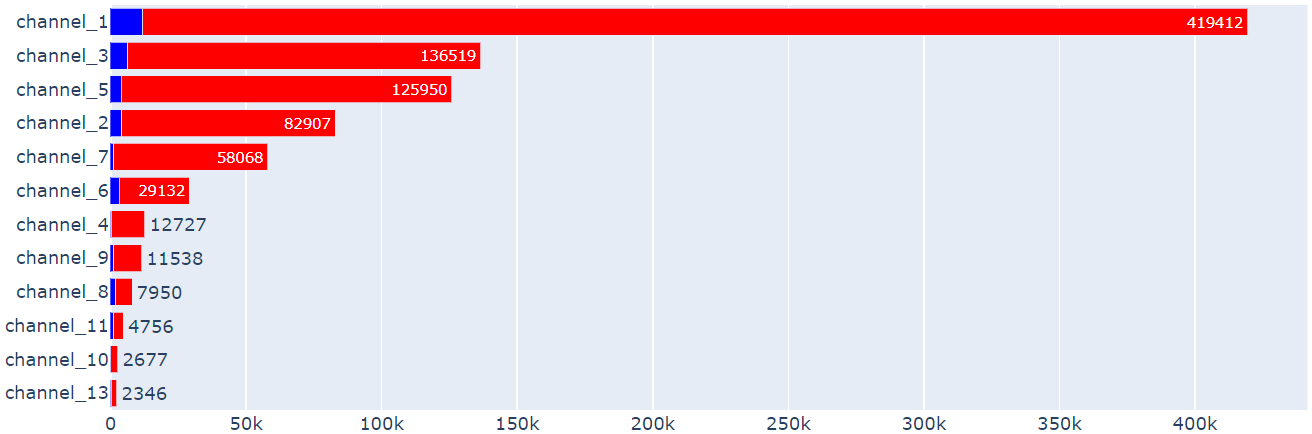
\includegraphics[width=16cm]{images/chan1.png}
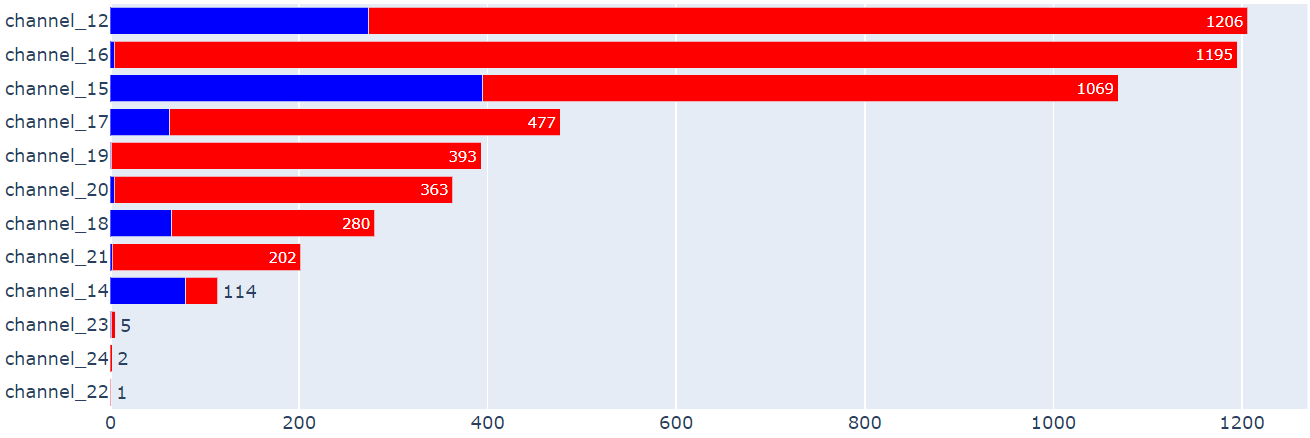
\includegraphics[width=16cm]{images/chan2.png}
\caption{Channel Occurences}
\label{fig:channel1}
\end{figure}
Upon examining the distribution of these channels across customer journeys, it becomes apparent that their occurrence does not follow a uniform pattern. Figure \ref{fig:channel1} illustrates this observation as it visualizes the number of channel occurrences across all customer journeys (not counting duplicates per customer journey) in a histogram. It's evident that some channels are encountered in only a handful of customer journeys, like channel\_22 which is only present in a single customer journey, while some other channels are remarkably prevalent, being observed several hundred thousand times.\\

Furthermore, Figure \ref{fig:channel1} divides the bars into a blue part, representing those customer journeys that ended in a transaction, and a red part representing the remaining customer journeys for which no conversion was documented. It is noteworthy that across nearly all instances, the red portion of the bars surpasses the blue counterpart with channel\_14 being the only exception there. However, it is important to highlight that for all channels the relative proportions between these two categories vary.

\begin{figure}[h]
\centering
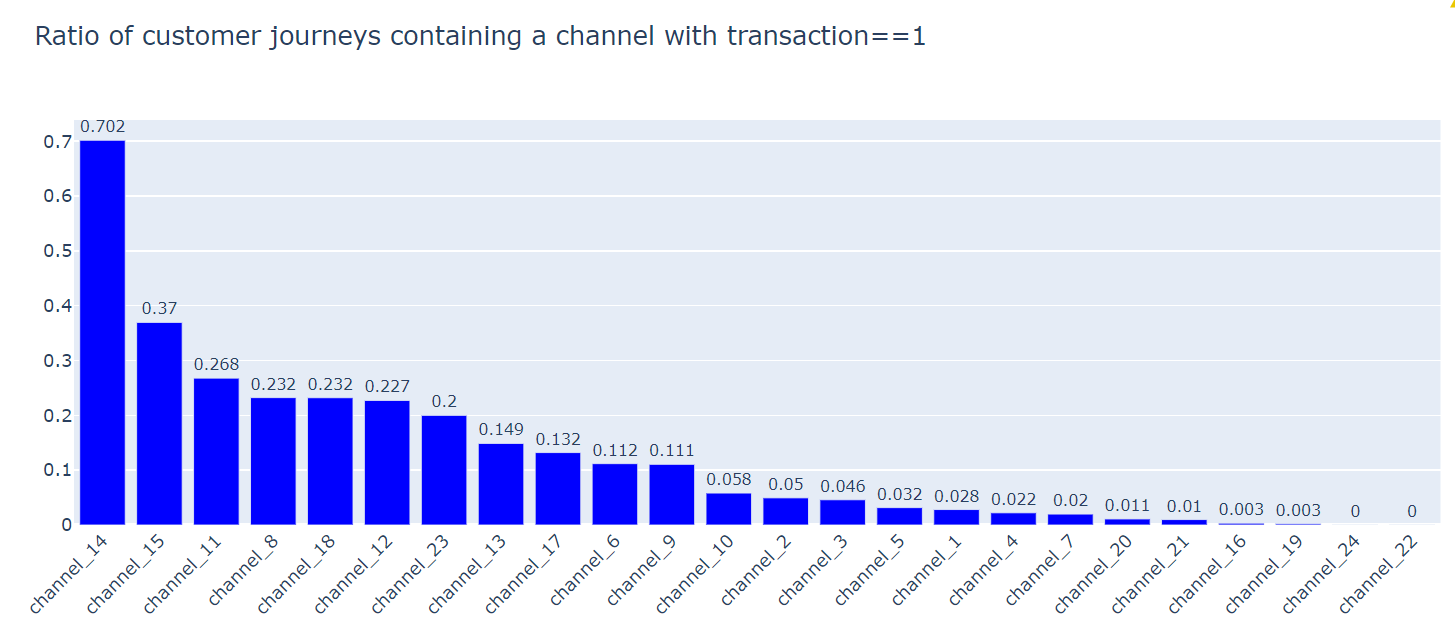
\includegraphics[height=7cm]{images/ratios_new.png}
\caption{Ratios}
\label{fig:ratio}
\end{figure}

To further explore these proportions, in Figure \ref{fig:ratio} the ratio of customer journeys containing a channel that actually led to conversion is visualized. For example of all customer journeys that contain channel\_14 around 70\% led to conversion, while of the customer journeys that contained channel\_10 only about 5\% ended with conversion. \\
As a result of the multi-touch attribution model one would expect the obtained channel importances to reflect this distribution to some extent, while also containing some differences. \\

\begin{description}
    \item[Countries:]
\end{description}
Another variable that is recorded is the country, where the customer is located. A total of 233 different countries were observed in the dataset. The location is observed for each touchpoint separately and thus does not have to stay constant within a customer journey.

\begin{figure}[h]
\centering
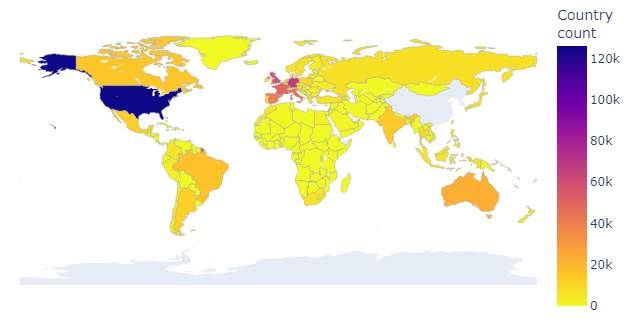
\includegraphics[height=7cm]{images/countrys.png}
\caption{Touchpoint location}
\label{fig:countrys}
\end{figure}

In Figure \ref{fig:countrys}, a visual representation of the global distribution of touchpoints is displayed. It's visible that touchpoints are dispersed worldwide, spanning from the United States to the Vatican, while China is a notable exception. This is surprising as there are offers for China on the GetYourGuide website but is probably caused by the censorship of the Internet in China and the common usage of VPN while traveling there and therefore masking China as the actual location. 
The United States boasts the highest number of touchpoints, closely followed by Western European countries, while the fewest touchpoints are found across Asia and Africa. \\
This does not represent the customer's nationality. As mentioned in the chapter introduction the data stems from an online travel agency therefore it's very possible that customers are traveling when exposed to a touchpoint.

\begin{description}
    \item[Platform:]
\end{description}
The variable \textbf{platform} holds information on the devices the touchpoint recorded on. The four possible expressions for this feature are \textit{mobileWeb}, \textit{desktop}, \textit{android}, and \textit{ios}.  

\begin{figure}[h]
\centering
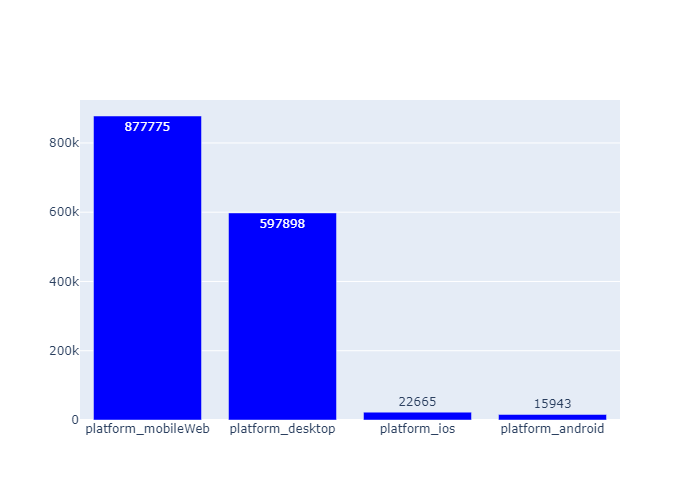
\includegraphics[height=7cm]{images/platforms.png}
\caption{Platform}
\label{fig:plattform}
\end{figure}

In this Histogram \ref{fig:plattform} one can observe two groups forming. \textit{mobileWeb} and \textit{desktop} are both in a similar range and together represent the majority of all touchpoints. On the other hand \textit{ios} and \textit{android} are also in a similar range but together only represent around 2.5\% .\\

With the available features we have no information on the customers or any other brand interactions such as click events, therefore no causal model could be implemented for this data. 

\section{Data Transformation}

The data set previously has been used for a different MTA approach, and thus some transformation is necessary to make it compatible with the phased GRU network. 
In the previous section already some changes to the data set were established with which we continue to work. 
Even though we said to remove the \textit{journey\_id} we will still use it for the transformation as an identifier in this section. 
The first transformation is to create dummy variables for the categorical variables \textit{channel, platform} and \textit{country\_name}. A dummy variable is created by replacing the variable column with columns for each possible expression of this variable. Each of these newly created columns is assigned '1' if a given observation expressed the respective categorical value and '0' else.\\
This greatly expands the size of the data set but is the best way to handle categorical data, that can not easily be transformed in an ordinal way. \\
The next transformation is to group together all touchpoints belonging to the same customer in order to form individual customer journeys. Previously the format of the dataset was in a table format \textit{touchpoint $\times$ features} where each row corresponds to a touchpoint observation with the observed features in the columns and the customer journeys aren't apparent. 
For the GRU network, we want to use customer journeys grouped together as one observation, which adds another dimension \textit{customer $\times$ touchpoints $\times$ features}. So for each customer $c$ with a customer journey of length $L$, we get $x_c=( f_l^T, t_l)_{l=1\cdots, L}$, where $f_l$ collects the recorded features of the $l$-th touchpoint, $t_l$ the timepoint of this touchpoint. We deliberately put the timestamp in the last position of the created tensor in order to extract the time by simply accessing the last position using the index "\textit{-1}". These timestamps are then used for the time gate. 
A problem that emerges with this approach are the varying customer journey lengths. While ragged tensors exist and could be used here to create tensors with an unspecified dimension size, ragged tensors are not very practical and cannot be used efficiently as of today. 
In an article \cite{patton-2022} presented an example that illustrates, that while using ragged tensors he was able to achieve marginally improved results but the computations for each training epoch took around 60 times more time compared to the same model trained with padded input. 
Therefore we also use padded input data, meaning all customer journeys get filled up with zeros to achieve the same length of 16. Here the decision to exclude long customer journeys proves to be helpful, as we don't have to artificially inflate the data set in order to keep all 3,143 touchpoints of the longest customer journey. \\
As target value, we use $y_c\in\{0,1\}$, the \textbf{transaction} for each customer which identifies two classes the successful and unsuccessful customer journeys. Therefore our prediction task is in fact a classification problem and we need to predict the class once per customer journey, at the end, when all touchpoints are considered. \\
The whole data is then split into a training and a test data set to appropriately fit and evaluate the model. 75 percent of customer journeys are randomly selected as training data in order to allow the model to learn well. 
The remaining 25 percent of the data is used to evaluate the predictions of the model after training is done. \\
Finally the data is split into batches of a fixed size to not overstrain storage space and achieve a faster training speed.\\

\chapter{The Model}
The proposed marketing attribution model is composed of two steps a phased GRU network for conversion prediction and  Shapley explanations for value attribution, which previously have been explained in detail.  
To test out the actual capabilities of this proposed multi-touch attribution model it has been realized in Python.\\
This chapter summarizes the actual realization of the phased GRU model in Python and the subsequent application of Shapley explanations. Before getting to the evaluation of the trained models a few metrics on which the model comparison is done are introduced. Finally, the trained phased GRU model will be compared to its counterpart without time gate as well as a basic and phased LSTM network.

\section{Implementation of phased GRU}
The implementation uses the Python TensorFlow library as the basis for the model, one of the main machine learning packages that are available for Python, that contains the necessary functions to create and train neural networks.\\
\begin{figure}[h]
    \centering
\begin{lstlisting}[language=Python]
modelphasedGRU = tf.keras.Sequential()

modelphasedGRU.add(
    tf.keras.layers.RNN(
        phased_GRUCell(...)
    )
modelphasedGRU.add(
    tf.keras.layers.RNN(
        phased_GRUCell(...)
    )
modelphasedGRU.add(tf.keras.layers.Dense(num_classes, activation='softmax'))
\end{lstlisting}
\caption{Network Structure}
\label{fig:network structure}
\end{figure}
While a tensorflow.keras.Sequential() model allows stacking several layers on top of each other the tensorflow.keras.layers.RNN() layer structure can be used to achieve a recurrent network layer that can process time series data and use the output of the current time step as input for the next time step. The actual phased GRU Cell that does all the computations in each time step, including the time gate calculations wasn't already available to use in this package and had to be separately implemented. \\
We use the source code of the basic GRU cell that can be found in the TensorFlow library \cite{unknown-author-2023} as a foundation from which the phased GRU cell class could be built by adding the time gate.\\
The phased GRU cell process one time step $l\in\{1,\cdots,16\}$ of a customer journey $c\in C$ at a time $x_{c,l}= (f_{c,l},t_{c,l})$. 
In order to implement the time gate, the time variable has to be extracted from the rest of the input. To access it, it has been placed as the last feature which can be referenced with the index $-1$ and stored separately from the other input variables. 
Then the necessary weights of the time gate are initialized as $\tau \sim \mathcal{N}^{p_l}(0,300),\ s\sim \mathcal{N}(0,3000),\ r_{on}\sim \mathcal{N}(0, 0.5),\ \tau \sim \mathcal{N}^{p_l}(0,300),\ \alpha\sim \mathcal{N}(0,0.5)$ as trainable parameters to get them in a range where they will end up. \\
The actual computations for the time gate are implemented as seen in \ref{fig:time gate} with one function determining the phase of the current time gate $\varphi$ and the other function returning the corresponding openness of the gate, and then using it to compute the hidden state. 
At the end of all the calculations within the phased GRU cell, if another phased GRUCell follows the current cell, the time variable has to be added to the output of this cell again, so the time gate in the next layer works properly. If it's the last phased layer, we have to make sure that it's not attached and returned to the next layer. 
In order to make sure everything is functioning properly the phased GRU Cell object class is created with two additional boolean parameters:
\begin{description}
    \item[time\_gate] \textit{True}: to use the time gate; \textit{False}: to use the Cell as a basic GRU Cell without a time gate
    \item[last\_layer] only needed if \textbf{timegate == True}; \textit{True}: if next layer uses a time gate and the time needs to be passed onto the next layer; \textit{False}: if the next layer has no time gate
\end{description}

\begin{figure}[h]
    \centering
\begin{lstlisting}[language=Python]
def phi_fast(time, s, tau):
    x = time - s
    x = tf.math.floormod(x, tau)
    x = tf.math.divide(x, tau)
    return x

def time_gate_fast(phi, ron, alpha):
    cond_1 = tf.cast(tf.less_equal(phi, 0.5 * ron), dtype='float32')
    cond_2 = tf.cast(tf.logical_and(tf.less(0.5 * ron, phi), tf.less(phi, ron)), dtype='float32')
    cond_3 = tf.cast(tf.greater_equal(phi, ron), dtype='float32')

    term_1 = tf.math.multiply(cond_1, 2.0 * phi / ron)
    term_2 = tf.math.multiply(cond_2, 2.0 - 2.0 * phi / ron)
    term_3 = tf.math.multiply(cond_3, alpha * phi)

    return term_1 + term_2 + term_3
    
\end{lstlisting}
\caption{Time gate}
\label{fig:time gate}
\end{figure}

As seen in \ref{fig:network structure} the actual model uses two phased GRU layers, followed by a Dense layer with softmax activation, returning a two-dimensional output $\hat{y}_c \in [0,1]^2$ with the first component $\hat{y}_{c,0}$ representing the predicted probability for no transaction and the second component  $\hat{y}_{c,1} = 1 - \hat{y}_{c,0}$ the probability for transaction.\\
As loss function we choose "sparse categorical crossentropy loss" as the true target values $y_c\in \{0,1\}$ are given as integer and the predicted labels as floating point values per possible output class $\hat{y}_c\in[0,1]^2$.  
In this case of binary classification the loss function returns:
\begin{align*}
    l(y_c, \hat{y}_c) &= - y_c \cdot \ln{(\hat{y}_{c,1})} - (1 - y_c) \cdot \ln{(\hat{y}_{c,0})}\\
&= \begin{cases}
     -\ln{(\hat{y}_{c,1})} \textrm{ , \ if } y_c=1 \\
     -\ln{(\hat{y}_{c,0})}  \textrm{ , \ if } y_c=0
\end{cases}
\end{align*}
This loss function penalizes wrong predictions very  harshly, as the function grows rapidly, if the model predicts the wrong class with high probability $-\ln(x) \xrightarrow{x\rightarrow 0} \infty $.\\
So the overall loss is computed as the average individual loss
\begin{align*}
    L = \frac{1}{C}\sum_{c=1}^C  l(y_c, \hat{y}_c) &= -\frac{1}{C}\sum_{c=1}^C  y_c \cdot \ln{(\hat{y}_{c,1})} +(1 - y_c) \cdot \ln{(\hat{y}_{c,0})}.
\end{align*}

The model will then be fitted on the training data set minimizing this loss function by using the adam optimizer to.
\color{red} explain adam optimizer \color{black}

\section{SHAP}
With the just created prediction model we now want to generate feature importances for the different marketing channels in the form of Shapley Additive exPlanations by using the shap library. \\
The shap package is the most commonly used Python library for XAI tasks as it unifies several different estimation approaches, for example \textit{TreeExplainer, DeepExplainer, PermutationExplainer, GradientExplainer,...}, that are optimized for a variety of different machine learning algorithms. The different explainer options provide global as well as local explanations and additionally offer easy comprehensible visualization options for the explanation model. 
\\ 
As we work with a deep learning model a DeepExplainer is the right explainer to use for the conversion prediction model, which is also used as the example explainer for an LSTM model on their official website
\footnote{https://shap.readthedocs.io/en/latest/example\_notebooks/text\_examples/sentiment\_analysis/\\Keras\%20LSTM\%20for\%20IMDB\%20Sentiment\%20Classification.html} and therefore should work for our model. 
But when applying it to the trained model one quickly realizes that this doesn't work as expected and throws errors left and right. 
Looking through the problem reports for shap on GitHub, a few issues regarding the compatibility of shap and TensorFlow can be found. There are two frequently suggested solutions, to downgrade TensorFlow to an earlier version, especially versions <2.0.0, where the shap package had no problem with a sequential model. However, the model is built on the newer contents of Tensorflow and is not easily transferable to an older outdated version. 
Another suggested solution is to flatten the input, which would mean all timesteps of a customer journey are combined into one long array. In this approach all timesteps would be processed at the same time, which would contradict the purpose of using a sequential model in the first place, and especially the time gate would be useless.\\
The most recent similar problem report is issue 3344 \footnote{https://github.com/shap/shap/issues/3344} from October 16th where a user encountered the same problem of not being able to generate shap explanations with the DeepExplainer for his LSTM network. A contributor of the package acknowledged the problem with the package and said he would look into solutions and update the problem report when a fix is found, which as of now \color{red}(17.11.2023) \color{black} is not the case.\\
As the other explainers in the package don't work as well, the only way to get shapley explanations for our model would be to implement something ourselves, which would exceed the scope of this thesis. 

\section{Metrics}
To evaluate and compare the models we use a few different metrics, which will briefly be introduced so that we can concentrate on comparing the models in the next section. \\
We compute the loss function on the training and the test dataset separately. 
During training the the model parameters are adjusted so that the model fits the training data set best 


and the test loss or test error is a better estimate for the actual \color{red} !!! WAS?? \color{black} \\
We can lable a customer journey  a transaction at the end of a customer journey a positive result and consequently no transaction a negative result. 
Comparing the predicted and real labels of the test data set we can form a \textit{Confusion Matrix} (\ref{fig:conf_mat}):\\
\begin{figure}[h]
\begin{center}
\centering
\begin{tabular}{ |m{4cm}||m{2.8cm}|m{2.8cm}| } 
  \hline 
   & predicted: transaction (PP) & predicted:\hspace{1cm} no transaction (PN) \\ 
  \hline \hline
  actual:\hspace{2cm}  transaction (P) & True Positive (TP) & False Negative (FN) \\
  \hline
  actual:\hspace{3cm}  no transaction (N) & False Positive (FP) & True Negative (TN)  \\ 
  \hline
\end{tabular}
\end{center}
    \caption{Confusion Matrix}
    \label{fig:conf_mat}
\end{figure}
The True Positive and True Negative predictions combined form all correct classifications of the model. Calculating the percentage of correct predictions we obtain the accuracy of the model: $$Accuracy=\frac{TP+TN}{TP+TN+FP+FN}.$$
As in the last chapter discussed accuracy alone isn't expressive, especially with this very unbalanced dataset, a few other metrics we can calculate from this confusion matrix are 
$$Precision=\frac{TP}{PP}=\frac{TP}{TP+FP}$$
$$Recall=\frac{TP}{P}=\frac{TP}{TP+FN} = TruePositiveRate = TPR$$
and
$$FPR = FalsePositiveRate = \frac{FP}{N} = \frac{FP}{FP + TN}.$$
The precision returns the fraction of correct predictions when looking only on positive predicted. The recall is also called true positive rate, returns which fraction of actually positive observations have been identified as such by the model. The data set contains only very few actually positive observations therefore having a good recall is especially important to ensure the model learned something and not only predicts the negative class.  On the other hand the \color{red} false positive rate \color{black}\\
The predictions we obtain using the phased GRU and the three comparison models don't simply classify the observations as zero or one but return probabilities for each class. From those probabilities, a classification is made choosing the class for which the probability is higher. This requires testing if $\hat{y}_{c,1} > \hat{y}_{c,0}$ and as we only have two classes and the probabilities sum up to 1, that's equivalent to checking  $\hat{y}_{c,1} > \frac{1}{2}$. \\
In case we want to allow more or less positive predictions we can move this threshold. When we lower the threshold more observations will be put in the positive class, when raising it more will be put in the negative class. As we want the model to be very confident in the predictions observing the metrics for different thresholds makes sense. \\
In the receiver operating characteristic (\textit{ROC}) curve we plot the TPR against the FPR. A perfect classifier's ROC curve would stick to the top left corner of the $[0,1]^2$ square. While a model that classifies purely random would stick to the diagonal. Therefore a model whose ROC is below the diagonal should be scraped, as it performs worse than a random guess, and any model further in the top left corner should be preferred. To simplify the comparison of ROC curves we can calculate the area under the curve (\textit{AUC}) which takes values between 0 and 1. The better a model is the closer the AUC will be to 1.\\
Another similar metric that we will evaluate is the precision-recall (\textit{PR}) curve. In a similar fashion to the ROC curve, precision and recall for different thresholds are plotted against each other. Here a perfect model would stick to the top right corner and a random model's PR-curve would be constant \color{red} ??? \color{black} \\
We compute those metrics for the phased GRU and the three comparison models with our test data set in order to have a good basis on which we can compare the models.

\section{Evaluation}
In order to evaluate the prediction of the phased GRU model we compare it to other models with a similar structure to see how well it performs. 
The models used in the comparison are a phased LSTM and a basic GRU and LSTM network to see the effect of the time gate and see if LSTM networks, which are the predecessor of GRU networks and in general are expected to outperform GRU networks, actually work better in this application.\\
They all use two model specific layers (i.e. phased/basic GRU/LSTM layers), followed by a dense output layer with softmax activation which returns a two-dimensional output vector for each customer journey $\hat{y}_c = (\hat{y}_{0,c}, \hat{y}_{1,c})\in [0,1]^2$ predicting the probability for each class. \\
The models are fitted using the same set of hyperparameters seen in \ref{tab:hyperparam} on the training data set. 
\begin{center}
\begin{tabular}{ |m{4cm}|m{6cm}| } 
  \hline 
  Inputsize & (?, 16, 262) \\
  \hline
  First Layer size & 64 \\ 
  \hline
  Second Layer size  & 64 \\ 
  \hline
  Output size & 2 \\ 
  \hline
  Batchsize & 5000  \\ 
  \hline
  Epochs & 30 \\ 
  \hline
  Learning Rate & 0.01 \\ 
  \hline
  Loss function & sparse\_categorical\_crossentropy \\ 
  \hline
\end{tabular}
\label{tab:hyperparam}
\end{center} 
\vspace{0.5cm}
During the model fitting process, the weights, biases, and time gate parameters are updated successively to minimize the training loss. Each epoch involves using all batches once, representing a subset of whole the training dataset, \color{red} batch job \color{black}. Once all batches have been utilized, the epoch concludes, and both training and test loss are recorded before the next training epoch begins. In \ref{fig:trainloss} we see how the training loss changes over the epochs for all four models.\\
  

\begin{figure}[h]
\centering
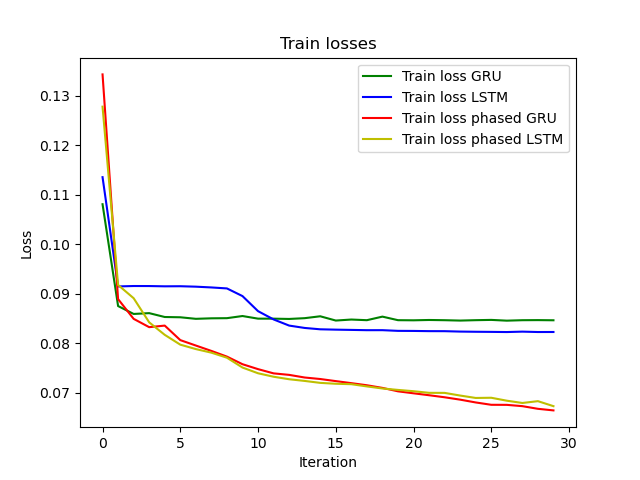
\includegraphics[height=10cm]{images/TrainingLosses_all.png}
\caption{Training losses}
\label{fig:trainloss}
\end{figure}
The training loss of the two models without time gate converges quickly after a few epochs the training error of the basic GRU model isn't changing significantly anymore, the training loss of the basic LSTM model does another significant jump down around the 10th epoch whereafter it remains pretty much constant and ends with a little lower loss than the GRU model. The time-gated models perform substantially better regarding the training loss. Not only do they end with a lower training loss, but after 30 epochs the loss still is decreasing for both models. \\
\begin{figure}[h] 
\centering
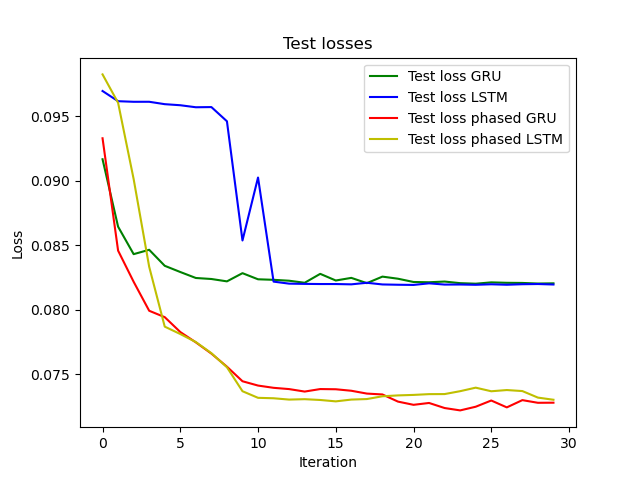
\includegraphics[height=10cm]{images/TestLosses_all.png}
\caption{Test losses}
\label{fig:testloss}
\end{figure}
\\
Similar development is displayed in the test loss. The networks with time gates perform notably better than the two models without. We see that the small jump in training error we observed in \ref{fig:trainloss} for the LSTM network around the 10th epoch corresponds to a huge decrease in test loss. 

Therefore we conclude a big effect of the time gate on the performance of the networks. 

All other metrics are calculated on the test data 
\begin{figure}[h]
\begin{minipage}[c]{0.5\linewidth}
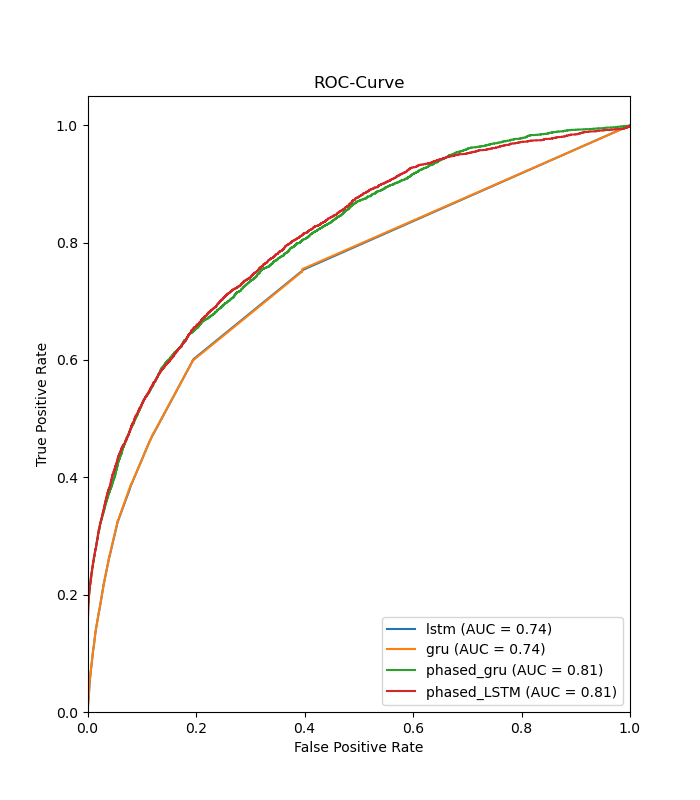
\includegraphics[width=\linewidth]{images/AUC_all.png}
\caption{ROC/AUC}
\label{fig:AUC}
\end{minipage}
\hfill
\begin{minipage}[c]{0.5\linewidth}
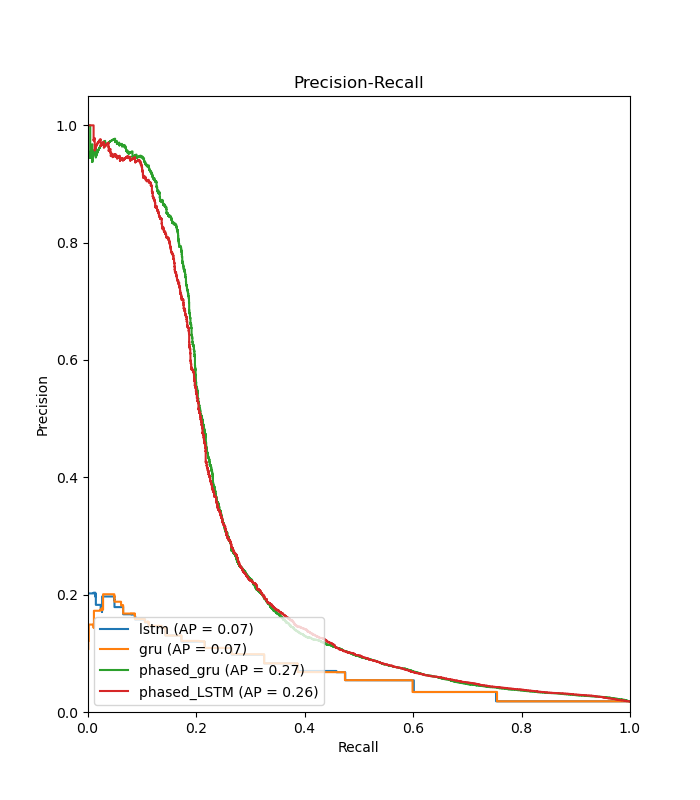
\includegraphics[width=\linewidth]{images/PR_all.png}
\caption{Precision Recall}
\label{fig:PR}
\end{minipage}%
\end{figure}


\begin{center}
\begin{tabular}{ |m{4cm}||m{2.5cm}|m{2.5cm}|m{2.5cm}|m{2.5cm}| } 
  \hline 
    & \textbf{phased GRU} & \textbf{GRU} & \textbf{phased LSTM} & \textbf{LSTM}\\ 
  \hline \hline
  trainable Parameters & \textbf{87,624} & 87,682 & 116,744 & 116,866 \\
  \hline
  Fitting time & 5011s &  \textbf{3910s} & 11808s & 5666s \\ 
  \hline
  Accuracy &  \textbf{0.98406} & 0.98178 & 0.98372 & 0.98178 \\ 
  \hline  
  Precision &  \textbf{0.78162} & - & 0.73281 & - \\ 
  \hline
  Recall & 0.17377 & - & 0.16726 & - \\ 
  \hline
  ROC-AUC & \textbf{0.81} & 0.74 &  \textbf{0.81} & 0.74 \\
  \hline  
  train loss &  0.06646 & 0.08467 & 0.06731 & {0.08230} \\ 
  \hline
  test loss &  \textbf{0.07277} & 0.08203  & 0.07300 & 0.08194 \\ 
  \hline
  minimal test loss &  \textbf{0.07218} & 0.08200 & 0.07287 & 0.08191 \\
  \hline
\end{tabular}
\end{center}




\chapter{Conclusion/Outlook}

\color{red} einordnung wie ob man das Model so verwenden soll\\
next steps \color{black} \\


As one can see, a phased GRU can predict conversion given a customer journey more reliably than the base GRU and LSTM models while using fewer parameters.\\ 

Obviously, the next step would be to add explanations to the model, whether it is using the shap package as soon as they are compatible with sequential data or to programming an own version that is compatible with the phased GRU model. 

Even though the predictions might be more accurate using neural networks, especially the phased GRU network, question still remains how much more and better information does such a model provide to a company compared to other simpler or easier interpretable models.


\bibliographystyle{apalike}
\bibliography{Quellen}


\begin{appendix}
\chapter{Appendix}
Collection of everything needed in this thesis, which would have disrupted the information presented. \\


LSTM?\\

ADAM?\\

Abkürzungsverzeichnis\\

KI-Tabelle

\end{appendix}


%\thispagestyle{empty}

\chapter*{}
\begin{center}
\large\textbf{Sworn Declaration}
\end{center}

\vspace*{1cm}
\onehalfspacing
\noindent

I hereby declare, that I have independently created the present work with the title\\

\begin{center}
[Title of the work]
\end{center}

any thoughts taken directly or indirectly from external sources have been identified as such. The work has not been submitted to any other examining authority or published before.

\noindent
I am aware that a false declaration may have legal consequences.

\vspace{3cm}
\noindent Ulm, den \today \hspace{4cm}\hrulefill\\
\vspace*{0.5cm}
\hspace*{10.0cm} (Leonie Allgaier)

%\newpage \vspace*{2cm} \pagestyle{empty}

${ } $



%%%%%%%%%%%%%%%%%%%%%%%%%%%%%%%%%%%%%%
%%%%%%%%%%%%%%%%%%%%%%%%%%%%%%%%%%%%%%
%%%%%%%%%%%%%%%%%%%%%%%%%%%%%%%%%%%%%%

\end{document}
